\section[动态实时定位]{动态实时定位\\Real-Time Kinematic Positioning}
Today most commercial applications of GPS are done in real time. Ten or twenty years ago it was common to collect data in the field and post-process them in the office. Postprocessing is nowadays only used for very accurate applications (geophysics and geodynamics). In meteorology one wants a processing delay of less than 90 minutes.

This section will describe aspects of a processing method that has been coined ��Real
Fime Kinematic�� (RTK). The method demands dual frequency receivers that output both
P code $P_{1}$, $P_{2}$ and phase observations $\Phi_{1}$, $\Phi_{2}$ on L1 and L2. The characteristic feature is that the processing takes place in real time , most often at the rover receiver. The baseline between master and rover is often determined at cm-level. Furthermore the method demands a data link that in real time transmits data or corrections from one receiver to the other. There are two restrictions on the distance between the master and the rover: The tromsmission link has to work at the longest distance, and the atmospheric parameters have to be correlated at the two sites. In practice this limit is about 10-20 km.

RTK is most often used by surveyors and they need the baseline to be known at the rover. So the master receiver data (or corrections) must be transmitted to the rover. The master can be a receiver run by the surveyor himself or for several surveyors. In some regions, companies run a set of master receivers and sell the data. The physical transmission link can be the internet combined with mobile telephony or a land mobile radio system.

We start by describing a standard format (RTCM) for transmission of data when the master and rover are not of the same make. For receivers of the same make you may stay with the internal binary data format that is proprietary for each manufacturer. Our sample
code includes binary formats , too.

\subsection{The RTCM Format}

The data transmission between master and rover is most often done via a telemetry link.A normal rate is 9600 bps or higher, and the format for the data transfer can be vendor dependent. However, a receiver independent RTCM format for this sort of data has now been developed, see RTCM (2004). The current version is 3.0, but 2.3 is still in use.

Table 10.4 lists the main data types defined. Types 18, 19, 20, and 21 are relevant for our purpose, more accurate than 10 and 11. A telemetry link demands line of sight between receivers, or signal repeaters at high points in the terrain. A more severe problem with data transfer in real time is the delay. The electronic delays in the system are caused by the distance between the receivers. The only solution is to predict what the observations would be at the rover site were they not delayed. Hence our method can only become a near real-time application . The computed position at the rover is only valid for the epoch time (increased by processing time).

\begin{table}[htbp]
	\caption{Message types in RTCM format}
	\newcommand{\tabincell}[2]{\begin{tabular}{@{}#1@{}}#2\end{tabular}}
	\begin{tabular}{ccc}
		\hline
		No.&Status&Description\\
		\hline
		1& fixed &differential GPS corrections\\
		2& fixed &delta differential GPS corrections\\
		3& fixed &GPS reference station parameters\\
		4& tentative &reference station datum\\
		5& fixed &GPS constellation health\\
		6& fixed &GPS null frame\\
		7& fixed &DGPS radiobeacon almanac\\
		8& tentative &pseudolite almanac\\
		9& fixed GPS &partial correction set\\
		10& reserved &P-code differential corrections\\
		11& reserved &C/A-code L1,L2 delta corrections\\
		12& reserved &pseudolite station parameters\\
		13& tentative &ground transmitter parameters\\
		14& tentative &GPS time of week\\
		15& tentative& ionospheric delay message\\
		16& fixed GPS &special message\\
		17& tentative& GPS ephemerides\\
		18& fixed RTK& uncorrected carrier phases\\
		19& fixed RTK &uncorrected pseudoranges\\
		20& tentative &RTK carrier phase corrections\\
		21& tentative &RTK high accuracy pseudorange corrections\\
		22& tentative& extended reference station parameters\\
		23-30& -& undefined\\
		31& tentative &differential GLONASS corrections\\
		32 &tentative &differential GLONASS reference station parameters\\
		33 &tentative &GLONASS constellation health\\
		34& tentative& GLONASS partial differential correction set ($N > 1$) ,\\
		&&GLONASS null frame ($N < 1$)\\
		35& tentative &GLONASS radiobeacon almanac\\
		36& tentative& GLONASS special message\\
		37 &tentative& GNSS system time offset\\
		38-58&- &undefined\\
		59 &fixed &proprietary message\\
		60-63 &reserved& multipurpose usage\\
		\hline
	\end{tabular}
\end{table}

\subsection{Description of RTK Code}

An RTK code includes recursive algorithms or filters to update the state vector for each
epoch. The filters may work on one - way, single or double differenced observations. The
more differencing used , the fewer entries in the state vector.

Most commercial software is based on double differences. This implies that the ambiguities in theory are integers. However, a new trend is to use single differenced and even one-way observation models. This makes sense when you have a detailed knowledge of the various error sources. For research purposes it is a big advantage to use one-way observations��allowing you to study or model any individual error.

Using double differences shortens the state vector x. It only contains baseline components,ionospheric delays, and integer ambiguities; but these observations are correlated.Single differences make it easier to introduce constraints, like I=0 for short baselines,and initial values for I that increase linearly with distance. The observations are uncorrelated.The state vector may have 50 entries.

We start by listing what an RTK software needs to do. This is valid for the ideal professional software as well:\\
1\,\,\,\,\,Get master observations $Obs_{1}$ from the first epoch
$$
Obs_{1}=
\begin{bmatrix}
P_{1}&\Phi_{1}&P_{2}&\Phi_{2}\\
\vdots&\vdots&\vdots&\vdots\\
P_{1}&\Phi_{1}&P_{2}&\Phi_{2}\\
\end{bmatrix}
$$
\,\,\,\,\,\,\,There are as many rows as there are tracked satellites in the epoch, say s.\\
2\,\,\,\,\,Check for cycle slips, reset of receiver clocks, and overall consistency between code
and phase observation. Here easy8 can be useful.\\
3\,\,\,\,\,For the first rover observations, check if the first epoch from master and rover are
identical. If not they have to be synchronized. Next find the set of PRNs common to the two receivers. If we know the ephemerides for four or more, we can compute all elevation angles, select
the reference PRN, and delete PRNs with elevation angle below a given threshold, say $10^{\circ}$.\\
\,\,\,\,\,\,\,Several things have to be tested from the very beginning, so it is not trivial to start   up all these functionalities. Missing data are appropriately substituted by 1*inf which
produces a NaN in MATLAB. This makes most MATLAB routines behave correctly.\\
4\,\,\,\,\,Compute WGS84 coordinates of master site $(X_{1},Y_{1},Z_{1})$. Convert to $(\varphi_{1},\lambda_{1},h_{1})$.\\
5\,\,\,\,\,Knowing $(\varphi_{1},\lambda_{1},h_{1})$ of the master and the measured antenna height $H_{1}$ we can compute the 3 by 1 offset vector u of the antenna center from the benchmark
$$
u_{1}=
\begin{bmatrix}
cos\varphi_{1}cos\lambda_{1}\\
cos\varphi_{1}sin\varphi_{1}\\
sin\varphi_{1}
\end{bmatrix}
H_{1}
$$
\,\,\,\,\,\,\,This procedure is repeated for the rover. The difference $up=u_{2}-u_{1}$ must be added to the estimated baseline.\\
6\,\,\,\,\,Set up filter for a priori baseline components (x,y,z)=(0,0,0) and variances.\\
7\,\,\,\,\,Find rover coordinates
$$
\begin{bmatrix}
X_{2}\\Y_{2}\\Z_{2}
\end{bmatrix}
=
\begin{bmatrix}
X_{1}\\Y_{1}\\Z_{1}
\end{bmatrix}
+
\begin{bmatrix}
x\\y\\z
\end{bmatrix}
$$
8\,\,\,\,\,To achieve $\varphi_{2},\lambda_{2},h_{2}$ of the rover receiver and compute the range between satellite and receivers we call\\
$[phi\_2,lambda\_2,h\_2]=togeod(a,f,X\_2,Y\_2,Z\_2);$\\
$[rho\_2\hat{ }k,X\_2,ECF]=get\_rho(time,Obs\_2,eph,(X\_2,Y\_2,Z\_2));$\\
$[rho\_1\hat{ }k,X\_1,ECF]=get\_rho(time,Obs\_1,eph,(X\_1,Y\_1,Z\_1));$\\
9\,\,\,\,\,Now we enter the main loop for s satellites, two receivers, and p epochs:

for $s = [PRNS]$

$[rho\_2,X\_2,ECF] = get\_rho(time,Obs\_2,eph,(X\_2,Y\_2,Z\_2))$;

$[rho\_1,X\_1,ECF] = get\_rho(time,Obs\_1,eph,(X\_1,Y\_1,Z\_1))$;

$A0 = [partials]$;

$[az,el,d]= topocent(X,X_ECF-X)$; \% four combinations

$t\_corr = tropo(sin(el * pi/180)$,$h_2 * 0.001,1013,293,50,0,0,0)\cdots $

$-tropr(\cdots)-tropr(\cdots) + tropr(\cdots)$;

$Phi\_1 = obsv1$;

$Phi\_2 = obsv2$;

$b = [PhM-lambda\_1 * N\_1; Phi\_2-lambda\_2 * N\_2-9$;

$b\_c = rho\_1\hat{ }s-rho\_2\hat{ }s-rho\_1\hat{ }t + rho\_2\hat{ }t$; \% double difference\\
end;\\
10\,\,\,\,\,if (first few epochs) and (probability $>$ 0.999999)

then

find ambiguities via accumulated normals by the Lambda or Goad method

else

filtering

end\\
11\,\,\,\,\,X=X+up

One way to process the data is through a filter for double differences. For centimeter accuracy the state vector must contain the coordinate differences (x,y,z) between master and rover, the L1 and L2 ambiguities, and for baselines longer than a few kilometers, also ionospheric delays l for each satellite. If a filter for single differences is preferred, augment the state vector with the receiver clock bias.

Double differenced data from s satellites in each epoch have 3 coordinate differences, and s-1 ambiguities on L1 and L2. Thus 2s+1 unknowns but only 2s observations. So initially we need at least two epochs for a meaningful estimation. After epoch 2 we have 4s observations and 2s+1 unknowns. To get initial values for the filter we collect observations from a few epochs and add them to a set of normals. The solution of these normals acts as the initial guess for the state vector. The next issue is to decide when to change non-integer ambiguities into integers. Teunissen (1998b) indicated how to compute the probability for finding the correct integers. As soon as this probability is larger than 0.99 we call lambda.

If everything works perfectly we now have a filter that runs smoothly and the changes in coordinates of the state vector are at mm level . However we have to specify covariances $\Sigma_{e}$ and $\Sigma\epsilon$ and $P_{0|0}$.

In the sequel we describe M -flies which perform RTK-like processing starting from stored data files,a situation that simulates data arriving in real time,and finally a start from RINEX files. All codes use double differenced observations.

\subsection{rtk1.m}

This real-time kinematic code processes data from Topcon receivers. The binary data are
stored in files 19 jan 07m.log and 19 jan07r.log. Below we comment on the code.

Handling of Ephemerides Data The GRIL format includes observations and ephemerides
in a continuous stream. They are transmitted in any order. Every ephemeris string has the
header GE.

The ephemerides are handled by allocating a 21 by 32 zero matrix . Each colum is related to a PRN. Every ephemeris is connected to the pertinent column. In case a new version of an already known ephemeris arrives we overwrite that column. This way the latest version of the ephemeris is stored in the matrix and can be read from it. This keeps the bookkeeping at a minimum.

Read Observation Files We open the master and rover files. We read epoch- wise one of the files repeatedly until the master and rover files are synchronous. (This step is not needed in a real-time set-up.) From L1 pseudoranges we compute the master position X\_i and convert to $(\varphi_{i},\lambda_{i},h_{i})$. Next we prepare for ambiguity estimation. The Goad method starts by accumulation of observations from the first no\_i epochs. The observation equation for each PRN is
$$
Ax=
\begin{bmatrix}
1&1&0&0\\
1&-1&\lambda_{1}&0\\
1&\alpha&0&0\\
1&-\alpha&0&\lambda_{2}
\end{bmatrix}
\begin{bmatrix}
\rho^{*}\\
I\\
N_{1}\\
N_{2}
\end{bmatrix}
=b
$$
with $\alpha=(f_{1}/f_{2})^{2}$. The weight matrix is C=diag($\sigma^{-2}$) with $\sigma^{2}=0.3m^{2}$ for pseudoranges and $\sigma^{2}=0.005m^{2}$ for phases. We accumulate the normals over time: A is constant over epochs and the right side b is accumulated by running over an outer loop $1:no\_i$ and an inner loop over all PRNs . The formal solution is
$$
x=(A^{T}CA)^{-1}A^{T}Cb
$$
For each satellite this yields two reals $x_{3}=n_{1}$ and $x_{4}=n_{2}$ from which we have to recover two integers $N_{1}$ and $N_{2}$. The estimated difference $n_{1}-n_{2}$ is rounded to the nearest integer and named $K_{1}$. The rounded value of $60n_{1}-77n_{2}$ we call $K_{2}$. The best integer estimates for $N_{1}$ and $N_{2}$ are then found as the solution
$$
\hat{N_{2}}=(60K_{1}-K_{2})/17
$$
$$
\hat{N_{1}}=\hat{N_{2}}+K_{1}
$$

The values for $K_{1}$ and $K_{2}$ are not free of error, but only particular combinations yield integer solutions for $N_{1}$ and $N_{2}$. Gradually these estimates improve as more epochs
are processed. The numbers $K_{1}$ and $K_{2}$, in theory, become more reliable.

The M-file goad selects the PRN with largest elevation angle as reference PRN for
the double differencing operations.

We prepare for the position filter with state vector (x,y,z,cdt):

\% Preparation for position filter

$P = 10\hat{} 8 * eye(4)$;                  \% covariances for state vector

$Q = 0.05\hat{} 2 * eye (4)$;               \% covariances of system

$R = 0.005\hat{} 2 * inv(Sigma)$;           \% covariances of observations

$A = []$;

$p = 0$;                             \% number of epochs processed

x = zeros (4,1);\\
The rover coordinates are set equal to the master coordinates. After these preparations we
are ready to start the epoch-by-epoch processing.

When reading observations, we substitute a missing observation by NaN. A NaN is simple to handle in MATLAB. The NaN test is performed for both master and rover data.

A rising PRN most often will start being observed at different epochs at master and
rover. We delete observations at one receiver until the PRN generates observations at both receivers. So we test if a new PRN really is present. If yes, we need to estimate the
ambiguities anew, as the additional unknowns $N_{1}$ and $N_{2}$ must be assigned correct values.

The sequence of PRNs at the master and rover receivers must be identical. We choose
to sort the PRNs in increasing order. (Alternatively you could reorder, the rover data to
match the master data.)

With a preliminary receiver position, the M-file get\_rho computes, in the ECEF system, the geometric distance between PRN and receiver. Then the entries of the A matrix can readily be computed.

For each PRN we compute the elevation angle needed for the tropospheric delay and an element of b is computed. Then we activate the extended Kalman filter:

\% Extended filter, see "Algorithms for Global Positioning" page 240f

$P = P+Q$;

$K = P*A' * inv(A*P*A'+R)$;

$x = K*b$;

$X\_j = X\_j + x$;

$P = (eye(size(x,1)) - K*A)*P$;

Recall, the important output of the filter is the baseline components.

\subsection{rtk2. M}

This code processes data from Ashtech Z12 receivers. The Ashtech data are stored in two
binary data files (b0810a94.076,b0005a94.076) , an ephemeris file (e0810a94.076),and two site files (s0810a94.076,s005a94.076). The M-file bdata.m reads the binary observation files and outputs them to an intermediate file bdata.dat.The M-file edata.m reads the ephemerides and stores the output in edata.dat. Finally the M-file sdata. m reads the two site files and writes the antenna heights into sdata.dat.

In most respects the code is similar to the rtk1 code. The ambiguities are estimated
by using the Goad algorithm.

\subsection{rtk3.m}

This code is our most comprehensive and flexible code for baseline estimation. We offer four sets of RINEX files which do not have perfect data. The reader is welcome to experiment with the data sets and get insight into the multitude of difficulties such data can expose. The ambiguities are estimated by the LAMBDA method.

As always we bring the ephemerides file in order. This is done for example by the call rinexe ('pta.96n','pta. nav'). We start by analyzing the header of the observation file from the master receiver: anheader('pta.96o'). The output contains some or all of\\
L1,L2 Phase measurements on L1 and L2\\
C1 Pseudorange using C/A Code on L1\\
P1,P2 Pseudorange using P Code on L1 and L2\\
D1,D2 Doppler frequency on L1 and L2\\

Next we read the master observation file until we find the first epoch flag equal to 0. This
indicates static observations (flag2 means start of moving antenna, and flag 3 is new site occupation). The file fepoch\_0('pta.96o') compares epoch times in the master and rover files until they match. Then we read observations of NoSv satellites by

grabdata (fid1, NoSv1 , NoObs\_types1)

grabdata (fid2, NoSv2, NoObs\_types2)

The observations are transformed into equations which in turn contribute to the normals. Double differenced observations are highly correlated, but the technique described in Section 6.7 decorrelates them before adding to the normals. That is the only valid method for adding the individual contributions from a single observation. Finally the normals are solved to estimate the baseline components and the ambiguities.

In this code we deal with the antenna offsets in an untraditional way. A common procedure is to compute the baseline between the two antennas and correct for the antenna offset at each station. However we introduce a nominal phase center related to the actual marker by the offset vector dx=(dH,dE,dN). The vector dx is expressed in topographic coordinates but has to be converted to the ECEF system. Next we calculate the distance D from the nominal phase center rather than the marker point:
$$
D=||X_{sat}-(X_{marker}+dx)||
$$
The distance D has to be subtracted from the calculated pseudorange $\rho_{j1}$ when forming the right side. Let the observed pseudorange be $P_{1}$, and correct the calculated geometric distance from satellite j to phase center 1 by D:
$$
corrected_obsj1=P_{1}+(\rho_{j1}-D)
$$

The last step of setting up the observation equations and normal equations is quite complex. We do not want to omit any valid observation. In rtk2, the M-file ash\_dd shaped the observations by brute force, to include only those satellites observed in all epochs. Here a more general code includes all observations in the RINEX file from any epochs.

This flexibility implies that we must be very careful in building the normals. The first
three unknowns are coordinate increments dx, dy, and dz of the baseline; the subsequent unknowns are ambiguities. Each time we encounter a new ambiguity we allocate a new position and increment the number of unknowns by one. All the necessary bookkeeping is done by the M-file locate. The file accum0 adds the individual contributions from the observation equations to the normal equations.

\subsection{easy6e}

easy6e is the same as easy6 except here the Kalman filter uses an overweighting of the most recent data. This method is also called exponentially weighted recursive least squares, see Kailath \& Sayed \& Hassibi(2000).

We introduce a known scalar $\tau$ such that $0\ll \tau<1$. Then $\tau^{i-j}$ weights past data(when j is far from i) less heavily than recent data (j near to i). This enables an adaptive algorithm to respond to variations in data statistics by ��forgetting�� old data. Figure 10.9 shows the result using an age-weighted, extended Kalman filter. Without age-weighting, the same data would produce the plot in Figure 10.8.

The smaller $\tau$ is, the faster old observations are ��forgotten.�� We quote the core code of the algorithm:
\% The smaller tau is, the faster old observations are forgotten

$tau = .1$;

$age\_weight = exp(1/tau)$;

$\% Extended Kalman filter$

$P = P + Q$;

$K = P * A' * inv(A * P * A'/age\_weight + R)/age\_weight$;

$x = x + K * (b - bk)$;

$P = (eye(3) - K*A)*P/age\_weight$;

In retrospect it is tremendous to realize that most of the tricks (like $\tau$) and computational options to improve filters were described within a few years after Kalman��s landmark paper in 1960.

\begin{figure}
	\centering
	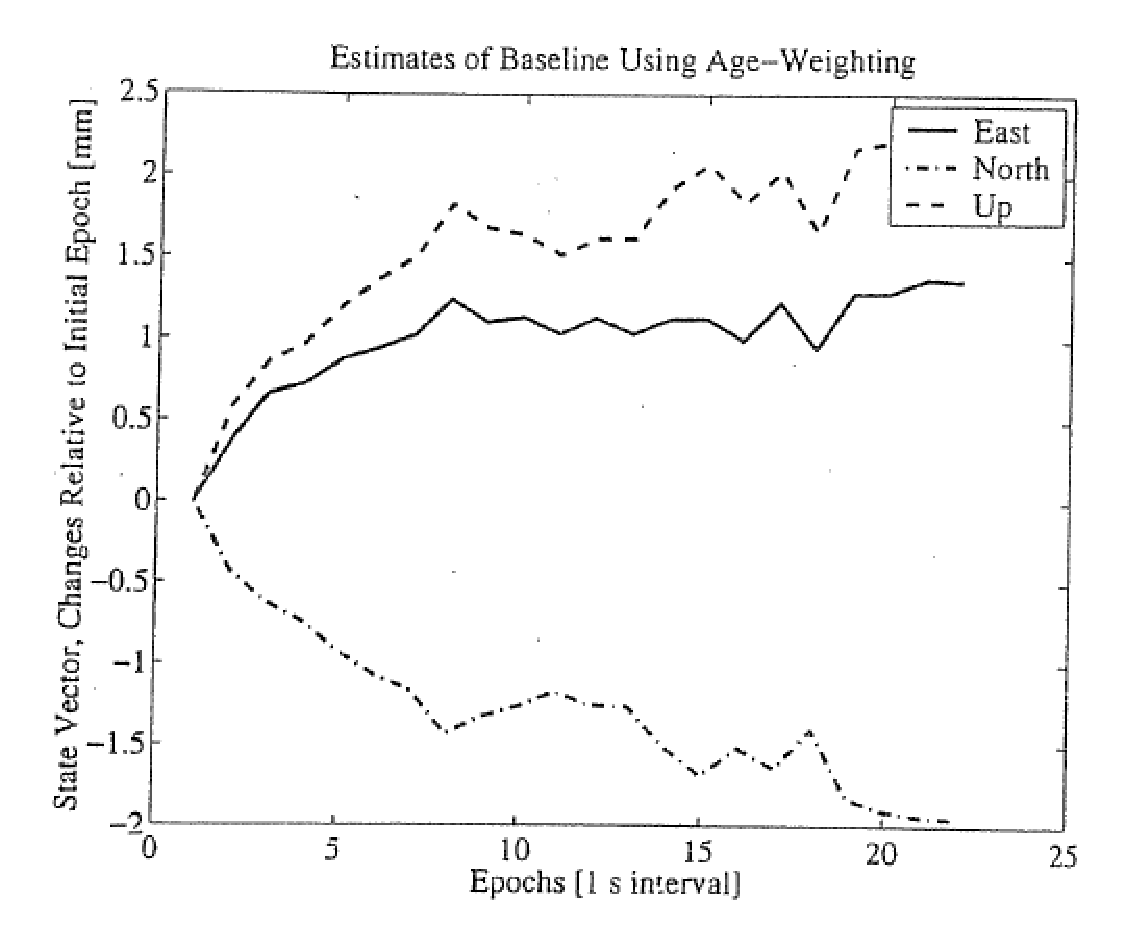
\includegraphics[width=0.4\linewidth]{TeX_files/Part03/chapter10/image/9-9}
	\caption{Baseline estimated by an age-weighted , extended Kalman filter.}
	\label{fig:9-9}
\end{figure}

\subsection{easy 9}

Textbooks on GPS do not make a big thing out of how to represent an estimated baseline. This is a pity because the subject is not trivial. If you want software that processes GPS data and also includes facilities for a surveyor, for example in setting-out problems , you need to analyze convergence of plumb lines and computation of height differences.

We restrict ourselves to the starting computations of station coordinates $P_{1}$ and $P_{2}$ with $P_{i}=(X_{i},Y_{i},Z_{i})$ and baseline length $||P_{2}-P_{1}||$ and given covariance matrix
$$
\Sigma_{XYZ}=
\begin{bmatrix}
\sigma_{X}^{2}&\sigma_{XY}&\sigma_{XZ}\\
\sigma_{YX}&\sigma_{Y}^{2}&\sigma_{YZ}\\
\sigma_{ZX}&\sigma_{ZY}&\sigma_{Z}^{2}\\
\end{bmatrix}
$$

Often we want the Cartesian coordinates converted to geographical $(\varphi,\lambda,h)$ coordinates.This is done by the togeod function.Consequently we also want to transform the covariance matrix $\Sigma_{XYZ}$ to an ellipsoidal covariance matrix $\Sigma_{\varphi\lambda h}$.

The transformation matrix is given in (9.20) as
$$
F=
\begin{bmatrix}
-sin\lambda&cos\lambda&0\\
-sin\varphi cos\lambda&-sin\varphi sin\lambda&cos\varphi\\
cos\varphi cos\lambda&cos\varphi sin\lambda&sin\varphi
\end{bmatrix}
$$

According to the law of variance propagation $\Sigma_{\varphi\lambda h}$. Furthermore we can convert the baseline components into Cartesian coordinates with origin at either $P_{1}$ or $P_{2}$.These topocentric coordinates can be represented either as 3-D Cartesian coordinates (E,N,U) or as spherical coordinates (Az,El,s):
$$
A_{z1}=arctan(E/N)
$$

\begin{figure}
	\centering
	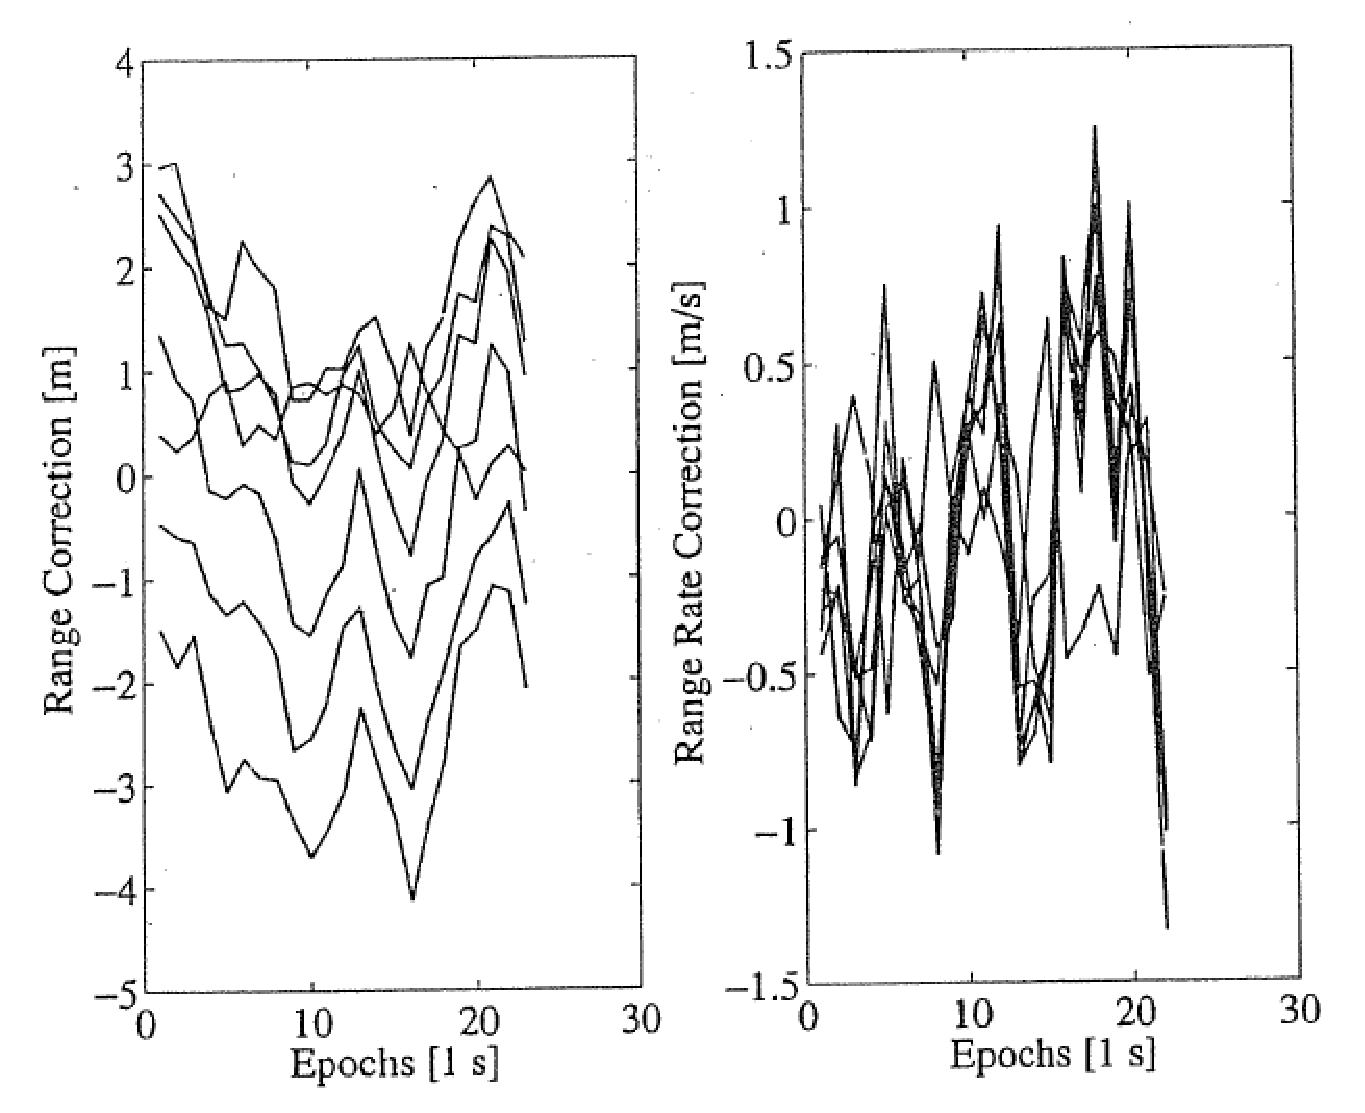
\includegraphics[width=0.4\linewidth]{TeX_files/Part03/chapter10/image/9-10}
	\caption{Range and range rate corrections as generated at a base station}
	\label{fig:9-10}
\end{figure}

$$
El_{1}=arctan(U/\sqrt{E^{2}+N^{2}})
$$
$$
s_{1}=\sqrt{E^{2}+N^{2}+U^{2}}
$$

Next we compute the geodesic between $P_{1}$ and $P^{}_{2}$.The classical computation yields the shortest distance $s_{12}$ between $P_{1}$ and $P_{2}$. We also get the azimuths at both terminals,and the height difference forward and reverse:$U_{1}=-U_{2}$

\subsection{easy18}

The first author was teaching GPS to control engineers working with air traffic. A need came up for computing range and range rate corrections at a base station.

We use the geometric distance $\rho$ between the satellite and the receiver antennas, the receiver clock offset $dt_{i}$, the satellite clock offset $dt^{k}$, and the tropospheric delay T . Then the corrected range is computed as
$$
\rho^{*}=\rho+cdt_{i}-cdt^{k}+T
$$
and the range correction as
$$
\delta=\rho^{*}-P_{obs}
$$
Figure 10.10 shows range and range rate corrections over 23 epochs using the September 4,2001 data. The receiver clock offset pos(4,:) varies between $1.13 \times 10^{5}$ and $1.15 \times 10^{5}$
through the 23s period of observations.